\section{Methods}

\subsection{Framework Overview}

The overall workflow of the proposed Sparse Transformer-based Explainable Hydrology (STEH) framework is illustrated in Fig.~\ref{fig:steh}. The framework provides an end-to-end interpretability pipeline for deep learning-based streamflow prediction, enabling systematic analysis from hydrological input variables, through internal neural structures, to prediction outputs.

The STEH framework consists of three main components: (1) sparse circuit discovery, (2) circuit verification and refinement, and (3) physical interpretation. Together, these components aim to reveal how deep learning models process hydrological information and whether the learned representations correspond to meaningful hydrological processes.

First, sparse circuit discovery is performed by introducing learnable gating mechanisms into the Transformer architecture. Gates are applied to input variables, attention heads, and feed-forward neurons, allowing the model to automatically identify a compact set of critical computational units during training. Through sparsity-inducing optimization, redundant structures are gradually suppressed, resulting in a sparse computational circuit responsible for streamflow prediction.

Second, circuit verification and refinement are conducted through systematic ablation experiments. Individual computational units—including input nodes, attention heads, and neurons—are selectively removed to measure their structural contribution to prediction performance. Units with negligible influence are discarded, yielding a compact core predictive circuit that preserves the essential functional structure of the model.

Third, the extracted core circuit is further analyzed to understand internal information flow and structural dependencies. Interaction analysis is used to identify cooperative or redundant relationships between model components. In addition, linear probing techniques are applied to hidden representations to evaluate whether internal states encode physically meaningful hydrological variables.

Finally, the interpretability results are validated from a hydrological perspective. Based on the structural knowledge extracted from the neural network, modifications are introduced to a Random Forest benchmark model to examine whether the discovered hydrological knowledge can improve data-driven hydrological simulations.

\begin{figure}[ht]
    \centering
    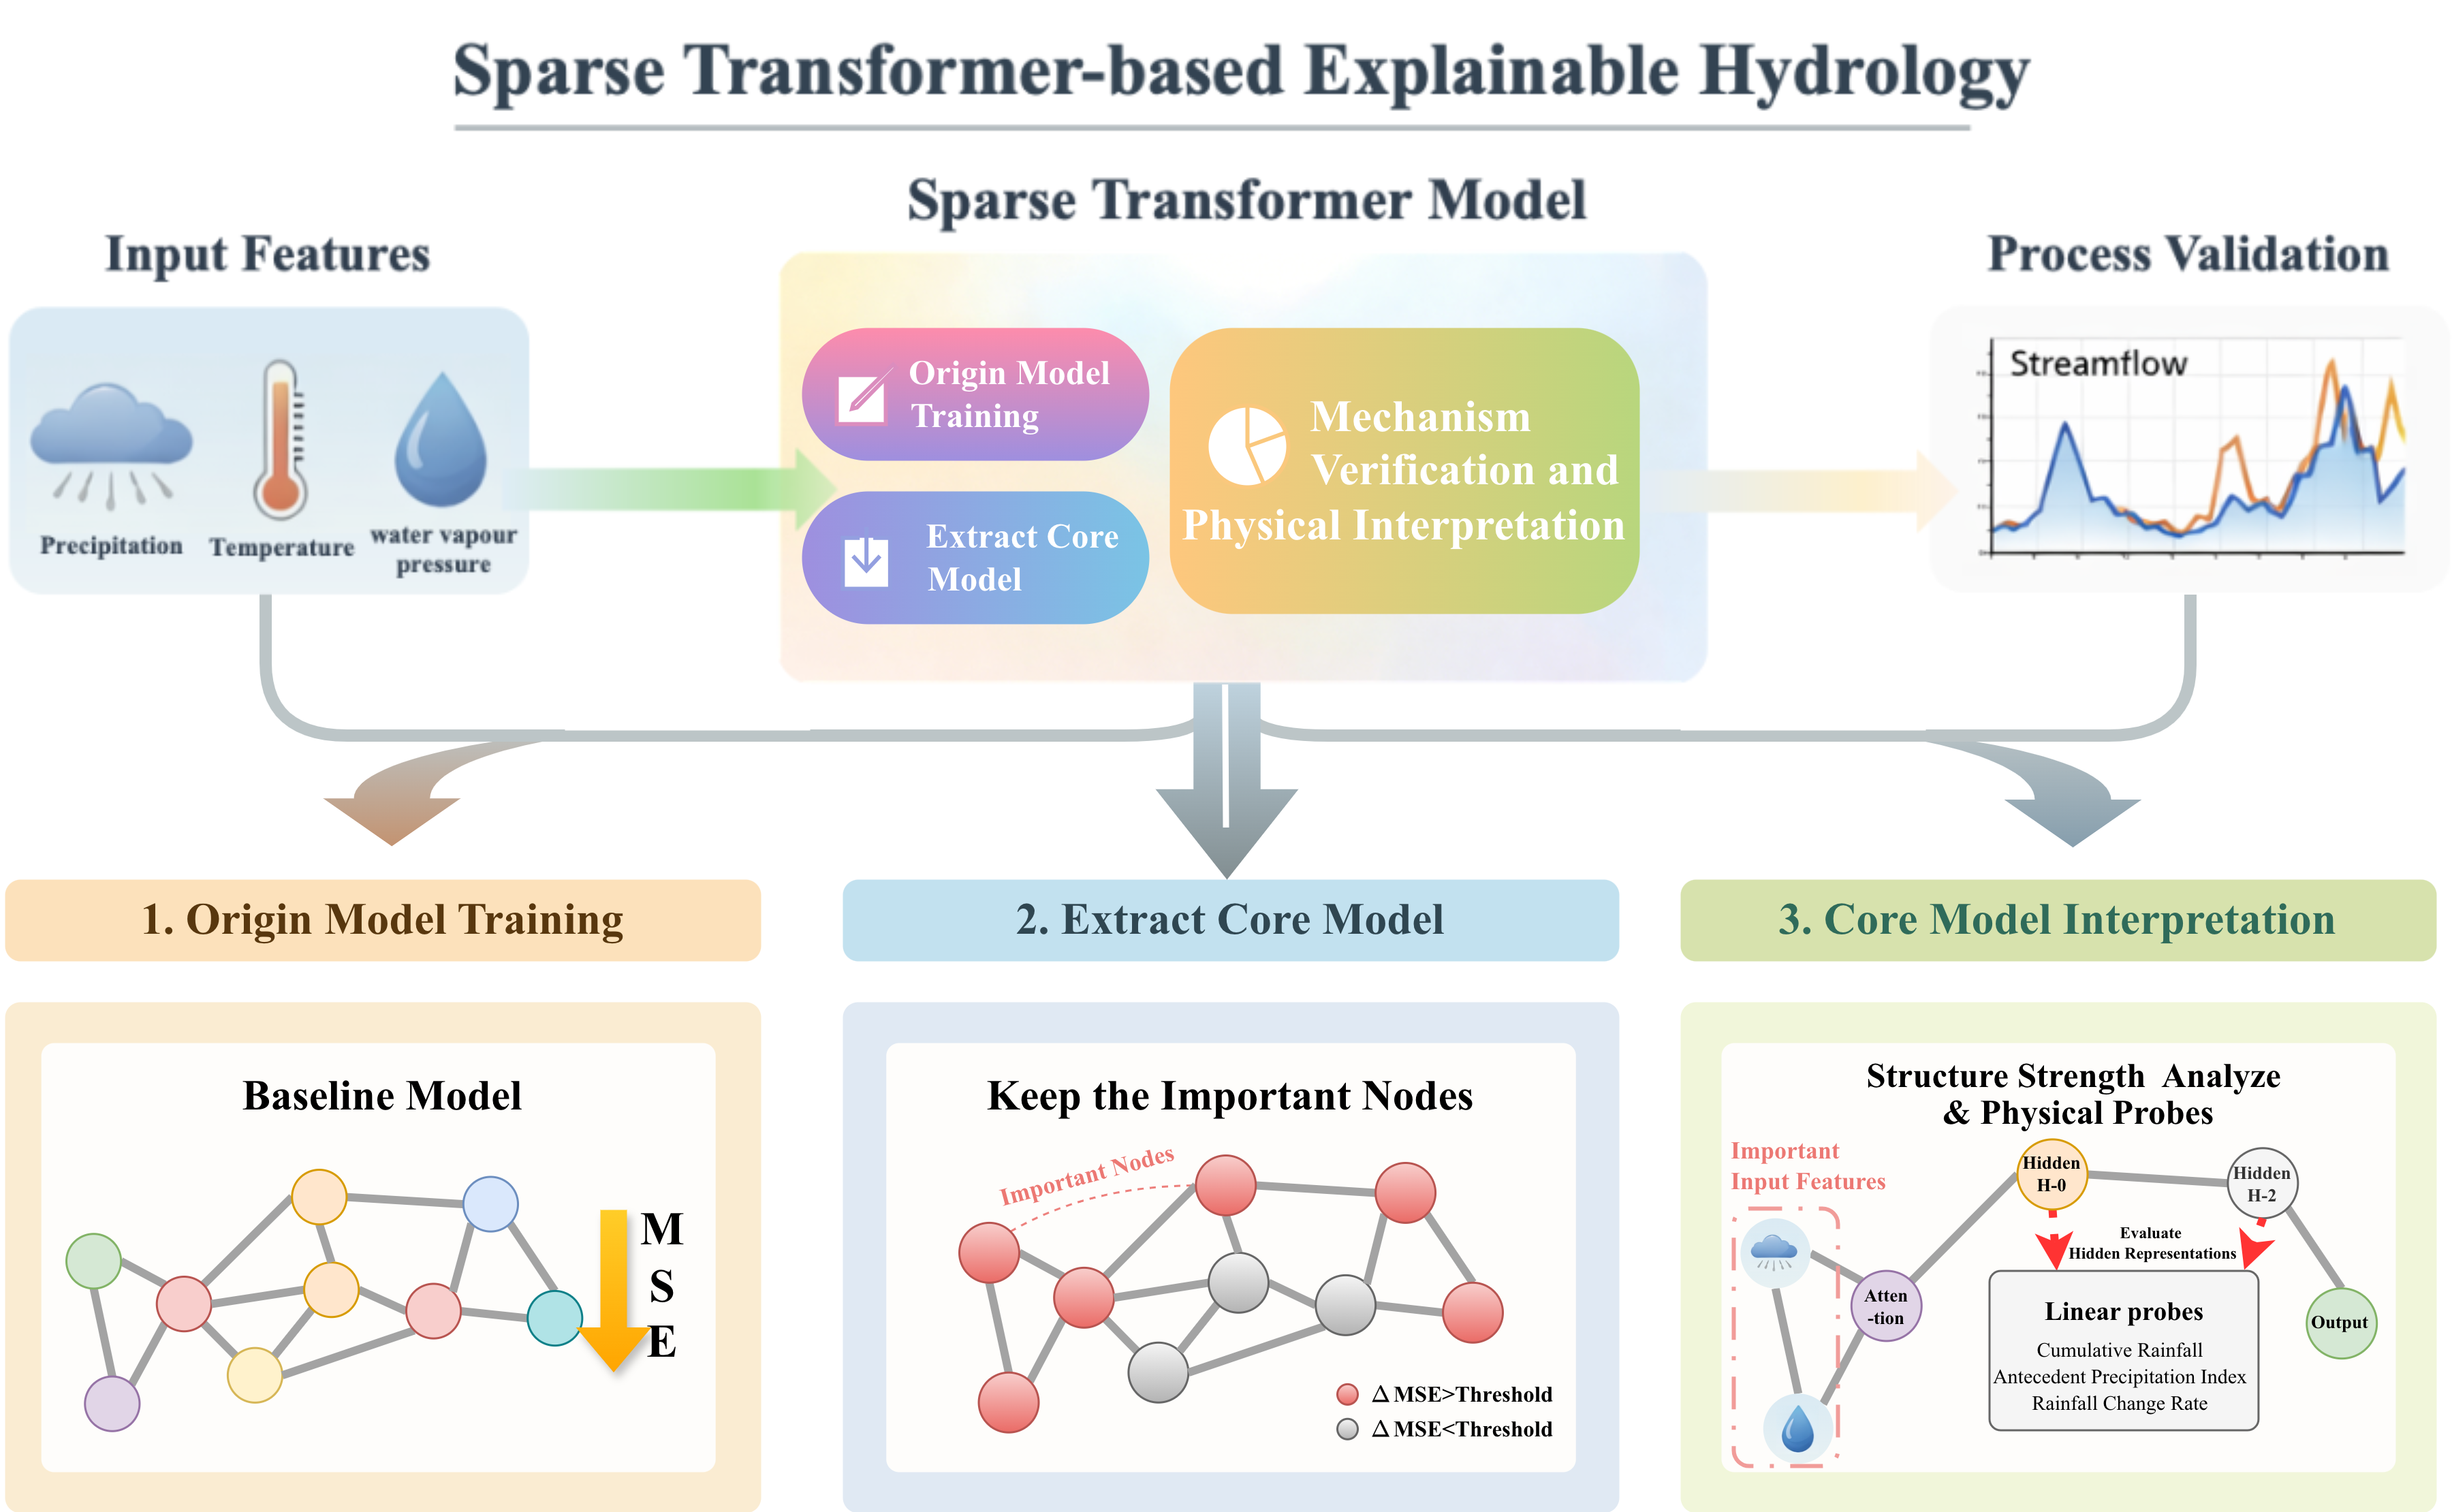
\includegraphics[width=\textwidth]{Figures/Fig1 MainStruct.png}
    \caption{Overall architecture of the proposed STEH framework}
    \label{fig:steh}
\end{figure}

\subsection{Sparse Transformer Architecture}

\subsubsection*{Transformer Formulation}

The Transformer architecture has recently been introduced into hydrological time-series modelling because its self-attention mechanism can effectively capture long-range temporal dependencies in hydro-meteorological sequences\cite{LIU2024131389}. In streamflow prediction, antecedent rainfall, temperature, and soil moisture conditions jointly influence discharge responses across multiple time lags, making long-term dependency modelling particularly important\cite{li2024application}.

Let $\mathbf{X}\in\mathbb{R}^{L\times F}$ denote the input sequence with length $L$ and feature dimension $F$. The self-attention operation is defined as\cite{dumontet2026_Transformer_nc}

\begin{equation}
    \mathrm{Attention}(\mathbf{Q},\mathbf{K},\mathbf{V})=
    \mathrm{softmax}\left(\frac{\mathbf{Q}\mathbf{K}^{\top}}{\sqrt{d_k}}\right)\mathbf{V},
\end{equation}
where $\mathbf{Q}$, $\mathbf{K}$, and $\mathbf{V}$ represent the query, key, and value matrices derived from the input representations, and $d_k$ denotes the key dimension used for scaling.

Hidden representations are updated through stacked Transformer encoder blocks\cite{AttentionIsAllYouNeed}:

\begin{equation}
    \mathbf{H}^{(l+1)}=\mathrm{Block}^{(l)}(\mathbf{H}^{(l)}), \quad l=0,\dots,N-1,
\end{equation}
where $\mathbf{H}^{(l)}$ represents the hidden state of layer $l$, and $N$ denotes the number of encoder layers.

\subsubsection*{Structured Gating Mechanism}

To enable circuit-level interpretability, structured gating mechanisms are introduced at three levels of the network architecture: input variables, attention heads, and feed-forward neurons\cite{louizos2018learningsparseneuralnetworks}. The effect of gate-based circuit selection is illustrated in Fig.~\ref{fig:sparseTransformer}(e--f).

For the input layer, the gated representation is defined as

\begin{equation}
    \tilde{\mathbf{X}}=\mathbf{X}\odot \mathbf{m}_{\mathrm{in}},
\end{equation}
where $\mathbf{m}_{\mathrm{in}}\in\{0,1\}^{F}$ is a binary mask indicating whether each input feature is retained.

Similarly, head-level and neuron-level masks are defined for each Transformer layer, denoted by $\mathbf{m}_{\mathrm{head}}^{(l)}$ and $\mathbf{m}_{\mathrm{neu}}^{(l)}$, respectively. These masks control the activation of attention heads and feed-forward neurons\cite{TFT}, enabling structured sparsification of the model.

\subsubsection*{Sparse Training Strategy}

Training is conducted in three consecutive stages to stabilize optimization and avoid premature pruning of potentially important connections\cite{NIPS2015_three_step_pruning}.

\textbf{Stage I (Origin Model Training).}
The model is first trained without sparsity constraints to establish a stable predictive baseline (Fig.~\ref{fig:sparseTransformer}(a--b)).

\textbf{Stage II (Weight Sparsification).}
Top-$K$ sparsity is progressively imposed on weight tensors with an annealed sparsity schedule\cite{zhu2017prunepruneexploringefficacy} (Fig.~\ref{fig:sparseTransformer}(c--d)):

\begin{equation}
    \rho_t=\rho_{\max}-(\rho_{\max}-\rho_{\min})\left(1-\frac{t}{T}\right)^{\gamma},
\end{equation}
where $\rho_{\min}$ and $\rho_{\max}$ denote the initial and final sparsity ratios. $t$ represents the pruning iteration, $T$ is the total number of steps over which sparsification is applied, and $\gamma$ is a shape parameter that controls the annealing schedule. Specifically, larger $\gamma$ values result in a slower increase in sparsity at early stages and a more rapid transition near the end, while smaller $\gamma$ leads to a more uniform sparsification process.

\textbf{Stage III (Mask Learning\cite{NEURIPS2019_1113d7a7}).}
Learnable gates are optimized with sparsity regularization (Fig.~\ref{fig:sparseTransformer}(e--f)):

\begin{equation}
\left\{
\begin{aligned}
\mathcal{L} &= \mathcal{L}_{\mathrm{task}}+\mathcal{L}_{\mathrm{gate}}, \\
\mathcal{L}_{\mathrm{task}} &= \frac{1}{M}\sum_{n=1}^{M}(\hat{y}_n-y_n)^2, \\
\mathcal{L}_{\mathrm{gate}} &= \lambda_{\mathrm{gate}}\frac{1}{|\mathcal{G}|}\sum_{g\in\mathcal{G}} p_g.
\end{aligned}
\right.
\end{equation}
where $M$ is the number of training samples in a mini-batch, $\mathcal{L}_{\mathrm{task}}$ is the mean squared error loss, $\mathcal{L}_{\mathrm{gate}}$ is the overall gate sparsity regularizer, $\mathcal{G}$ denotes all learnable gates. We consider two types of gates: input-level gates and node-level gates, corresponding to \textit{input} and \textit{head\_neu}, respectively, and $p_g$ is the activation probability of gate $g$.

\begin{figure}[ht]
    \centering
    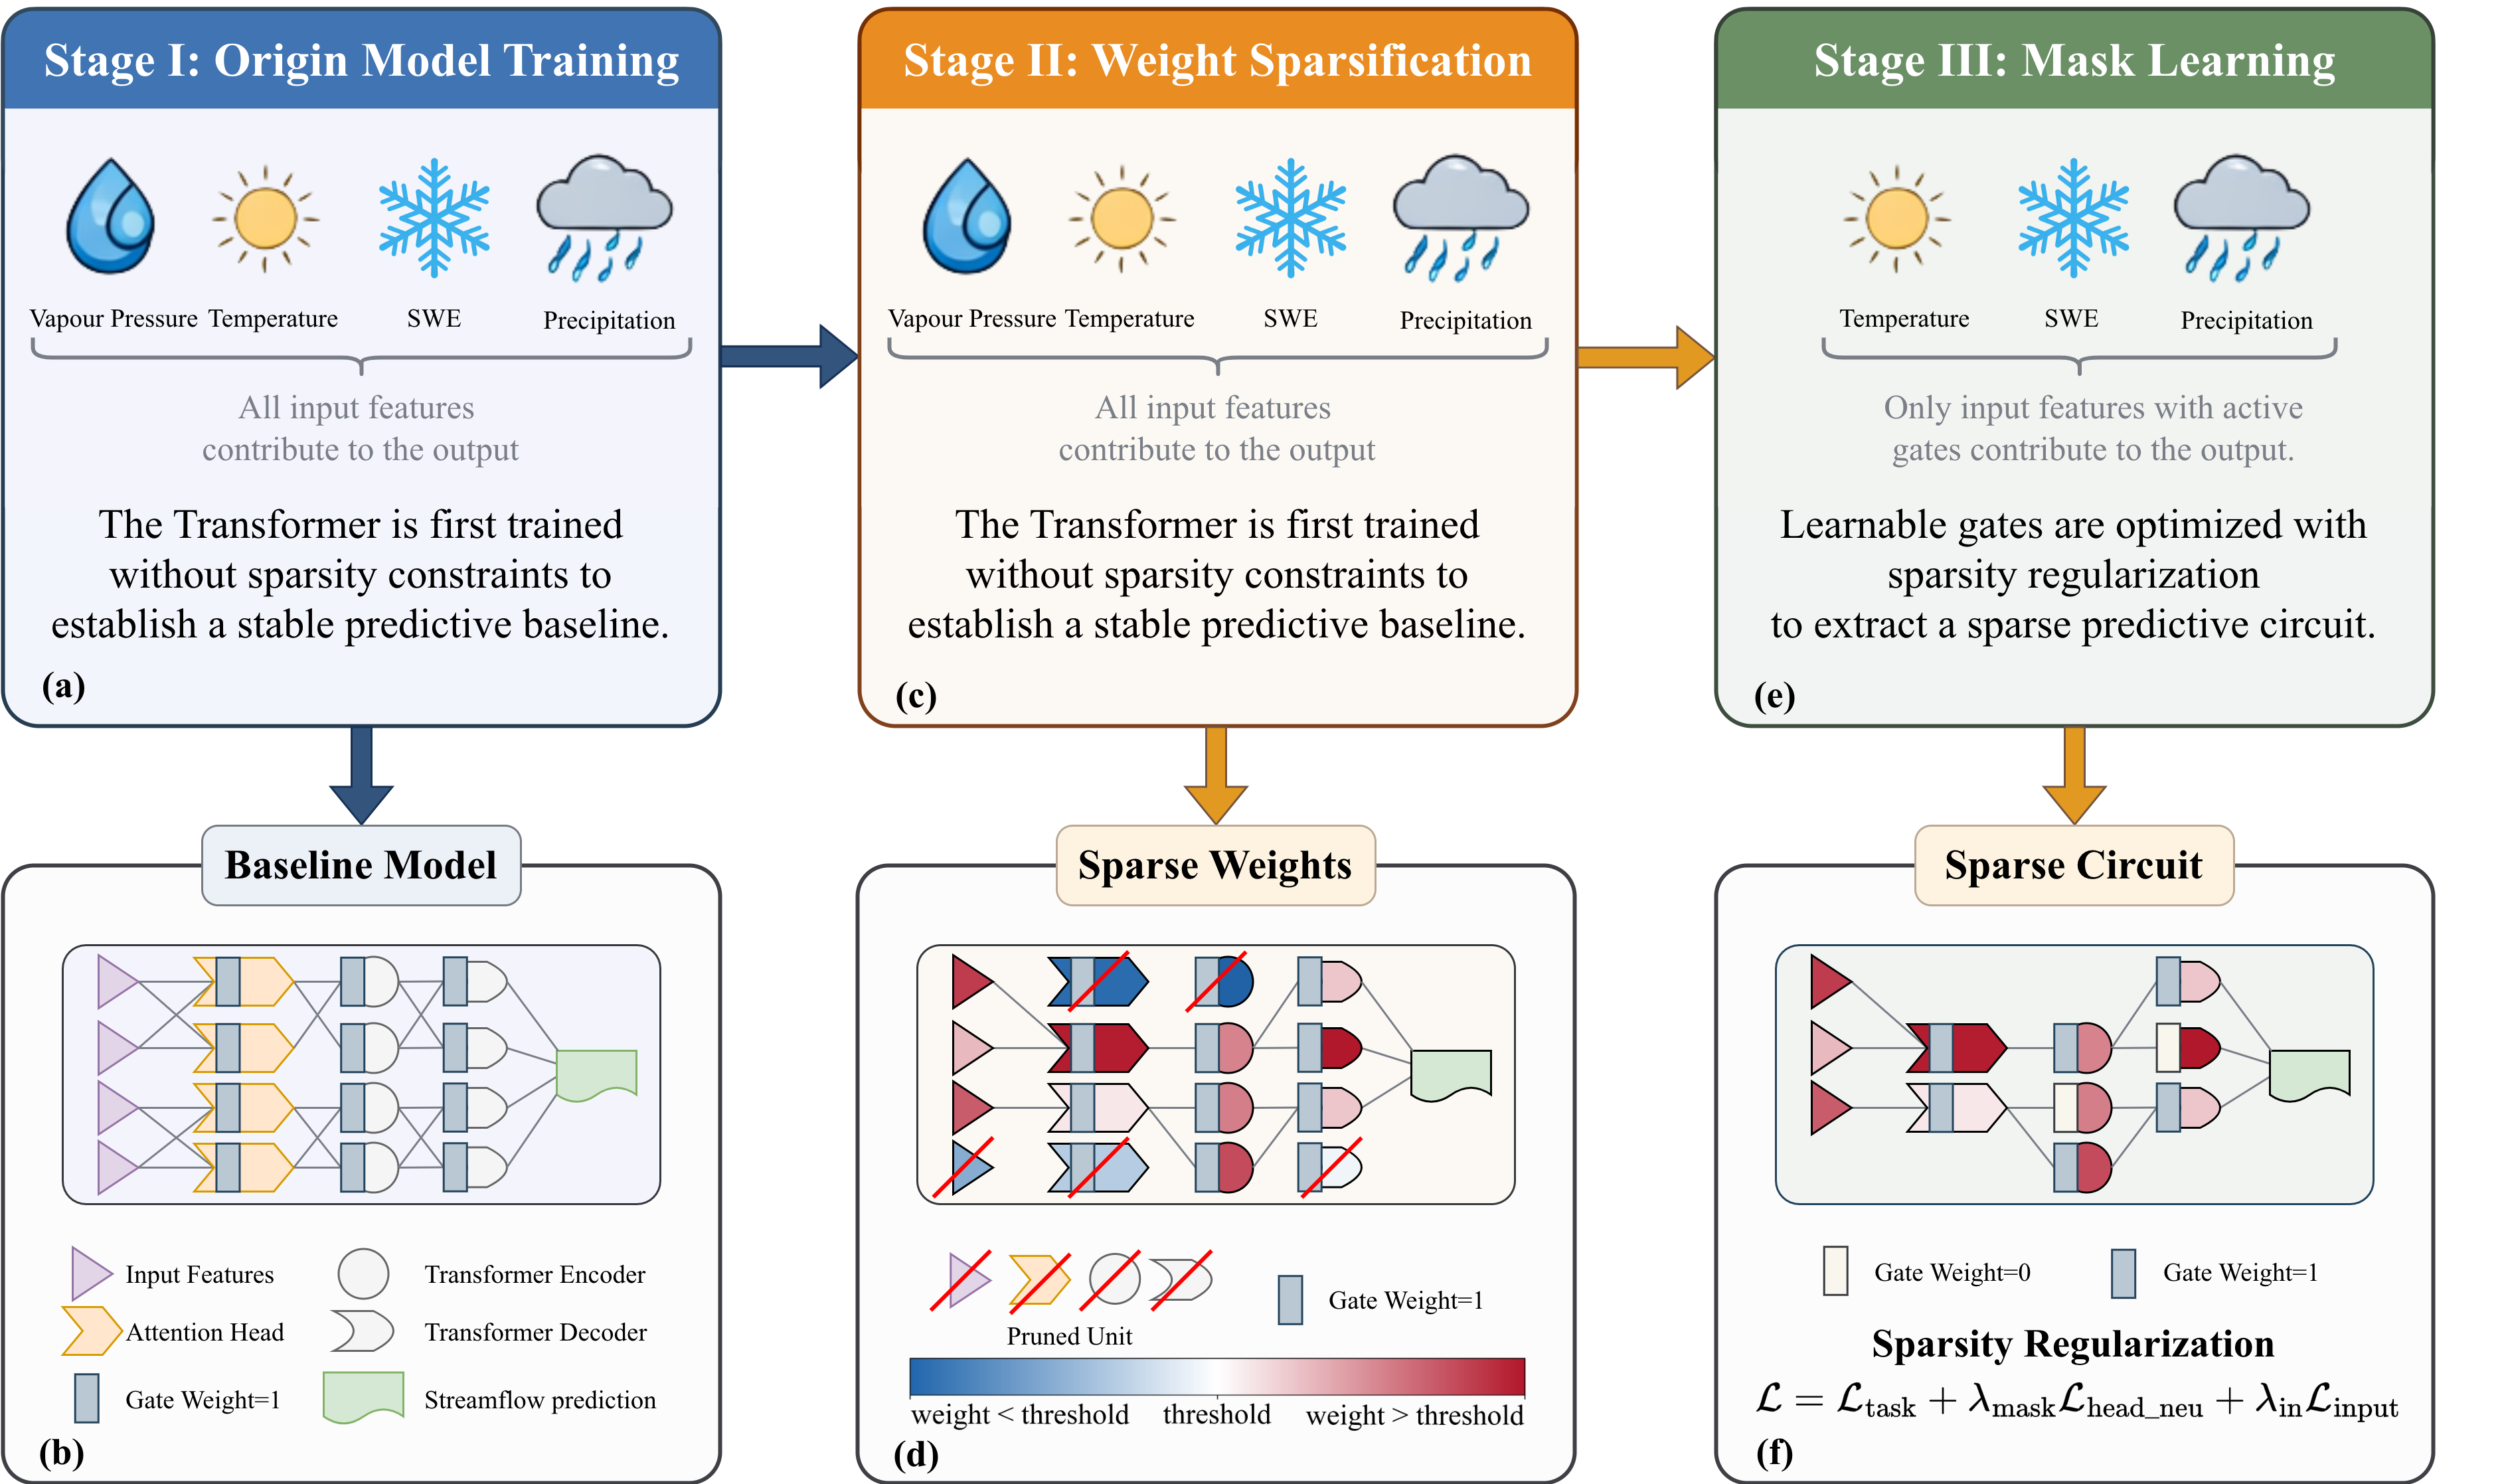
\includegraphics[width=\textwidth]{Figures/Fig2 ThreeStep.png}
    \caption{\textbf{Three-stage sparsification framework for predictive circuit discovery in Transformer.}
        The model is trained through three stages to progressively transform a dense Transformer into a sparse predictive circuit.
        (a–b) Stage I: Origin model training, where the Transformer is trained without sparsity constraints and all input features contribute to the prediction.
        (c–d) Stage II: Weight sparsification progressively prunes redundant connections according to the sparsity schedule.
        (e–f) Stage III: Mask learning optimizes learnable gates so that only a subset of input features contributes to the final prediction.
        For clarity, only a subset of connections between layers is illustrated in the figure, while the actual model remains fully connected, and decoder attention layers are omitted for simplicity.
        Note that the proposed method does not explicitly modify the network architecture; sparsity is achieved by setting weights or gates to zero, while the visual removal of units in the figure is only for illustrative purposes.
        The number of input variables shown in the figure is fewer than the actual input feature set; this simplification is adopted solely for visual clarity.
    }
    \label{fig:sparseTransformer}
\end{figure}

After training, a compact core predictive circuit is extracted by thresholding gate probabilities.\cite{openai_weight_sparse_transformers} Let $p_i=\sigma(z_i)$ denote the activation probability of gate $i$. A unit is retained if

\begin{equation}
    a_i=\mathrm{I}(p_i>\tau),
\end{equation}
where $\tau$ is the pruning threshold. Applying this rule to all gates yields a compact model containing only the most important computational pathways.

\subsection{Interpretability Analysis}

\subsection*{Ablation-based Importance}

To quantify the causal importance of individual computational units, targeted ablation is applied to each candidate unit $u$~\cite{morcos2018importancesingledirectionsgeneralization}. The importance score is defined as

\begin{equation}
    \Delta \mathrm{MSE}_{u}=\mathrm{MSE}(\mathrm{ablate}(u))-\mathrm{MSE}(\mathrm{base}).
    \label{eq:Delta_MSE}
\end{equation}

Unlike gradient-based attribution methods, this intervention-based measurement directly evaluates the causal contribution of each component by observing the performance change after structural removal\cite{wang2022interpretabilitywildcircuitindirect}.

\subsection*{Interaction Analysis}

To analyze dependencies between components, pairwise interaction scores are defined as

\begin{equation}
    I_{ij}=\Delta_{ij}-\Delta_i-\Delta_j.
    \label{eq:interaction}
\end{equation}

Positive values indicate synergistic interactions, whereas negative values suggest redundancy or functional substitution.

\subsection*{Top-K Faithfulness}

To evaluate the trade-off between circuit compactness and predictive fidelity, a top-$K$ faithfulness analysis is conducted by retaining only the most important units and measuring the resulting performance degradation\cite{7552539}.

\subsection*{Physical Probing}

To examine whether hidden representations encode physically meaningful hydrological information, linear probes are applied to hidden states\cite{pmlr-v97-verma19a}.

Let $\mathbf{h}_n\in\mathbb{R}^{D}$ denote the hidden representation of sample $n$. The probe model is defined as

\begin{equation}
    \hat{y}_n^{\mathrm{phys}}=\mathbf{w}^{\top}\mathbf{h}_n+b,
\end{equation}
where $\mathbf{w}$ and $b$ are parameters estimated using least squares regression.

Probe performance is evaluated using the coefficient of determination ($R^2$). To avoid probe overfitting, the probe model is intentionally restricted to a simple linear form without hidden layers.

Representative hydrological variables such as cumulative rainfall\cite{PIRONE2023128949}, antecedent precipitation index (API)\cite{CAMELS}, and rainfall change rate are used as probe targets. Let $P_t$ denote precipitation at day $t$, and let $W$ be the look-back window length. Their definitions are

\begin{equation}
    R^{\mathrm{cum}}_t(W)=\sum_{k=0}^{W-1} P_{t-k},
\end{equation}

\begin{equation}
    \mathrm{API}_t(W,\kappa)=\sum_{k=0}^{W-1}\kappa^{k}P_{t-k}, \qquad 0<\kappa<1,
\end{equation}

\begin{equation}
    R^{\mathrm{chg}}_t=\frac{P_t-P_{t-1}}{P_{t-1}+\varepsilon},
\end{equation}
where $\kappa$ is a decay factor controlling the memory of antecedent rainfall and $\varepsilon$ is a small constant to avoid division by zero.

\subsection{Evaluation Metrics}

Model evaluation is conducted from three perspectives: predictive accuracy, explainability properties, and hydro-climatic diagnostics.

Predictive accuracy is measured using standard hydrological metrics including RMSE\cite{WRR_RMSE}, MAE\cite{WRR_MAE}, and NSE\cite{WRR_NSE}. Explainability-related metrics include ablation importance ($\Delta\mathrm{MSE}$, Eq. ~\ref{eq:Delta_MSE}), interaction score ($I_{ij}$, Eq. ~\ref{eq:interaction}), and top-$K$ faithfulness\cite{7552539} trends. Structural sparsity statistics are also reported to quantify circuit compactness.

Hydro-climatic diagnostics are used to characterize the climatic regimes of catchments. Let $\bar{P}$, $\overline{\mathrm{PET}}$, and $\bar{Q}$ denote the long-term mean annual precipitation, potential evapotranspiration, and streamflow, respectively, and let $P_m$ ($m=1,\dots,12$) be the mean monthly precipitation with $\bar{P}_{\mathrm{ann}}=\sum_{m=1}^{12}P_m$.

The \textbf{aridity index} (AI)\cite{zomer2022version} describes the balance between water supply and atmospheric demand:
\begin{equation}
    \mathrm{AI}=\frac{\bar{P}}{\overline{\mathrm{PET}}}.
\end{equation}
Values $\mathrm{AI}<1$ indicate arid conditions, while $\mathrm{AI}>1$ indicates humid conditions.

The \textbf{Streamflow coefficient} ($C_r$)\cite{WRR_coefficient} represents the fraction of precipitation that becomes streamflow:
\begin{equation}
    C_r=\frac{\bar{Q}}{\bar{P}}.
\end{equation}

The \textbf{precipitation seasonality index} (SI)\cite{SI} quantifies the degree of seasonal concentration of rainfall:
\begin{equation}
    \mathrm{SI}=\frac{1}{\bar{P}_{\mathrm{ann}}}\sum_{m=1}^{12}\left|P_m-\frac{\bar{P}_{\mathrm{ann}}}{12}\right|,
\end{equation}
where $\mathrm{SI}=0$ indicates perfectly uniform monthly distribution and larger values correspond to stronger seasonal concentration. Together, these three diagnostics are used to stratify stations by hydro-climatic regime and to contextualize model performance across different environmental conditions.